% \section{Blockchain attributes}
% %Basic attributes of blockchains, an abstraction, blockchain as an idea.
% %Discussion about terminology as consortium over private etc. State of the industry
% An ever-growing distributed list of records, append only, replicated and shared among the participants of the network (aka distributed ledger). Each block in the chain contains a list of transactions and a hash of the previous block. Blockchain is a log whose records are batched into time-stamped blocks where each block is identified by its hash. By including the hash of the previous block\footnote{The Genesis block, is the first block on the chain and it does not include a reference to a previous block.}, it establishes a link between the blocks, thus creating a block-chain. 
% 	\begin{figure}[H]
% 	    \centering
% 	    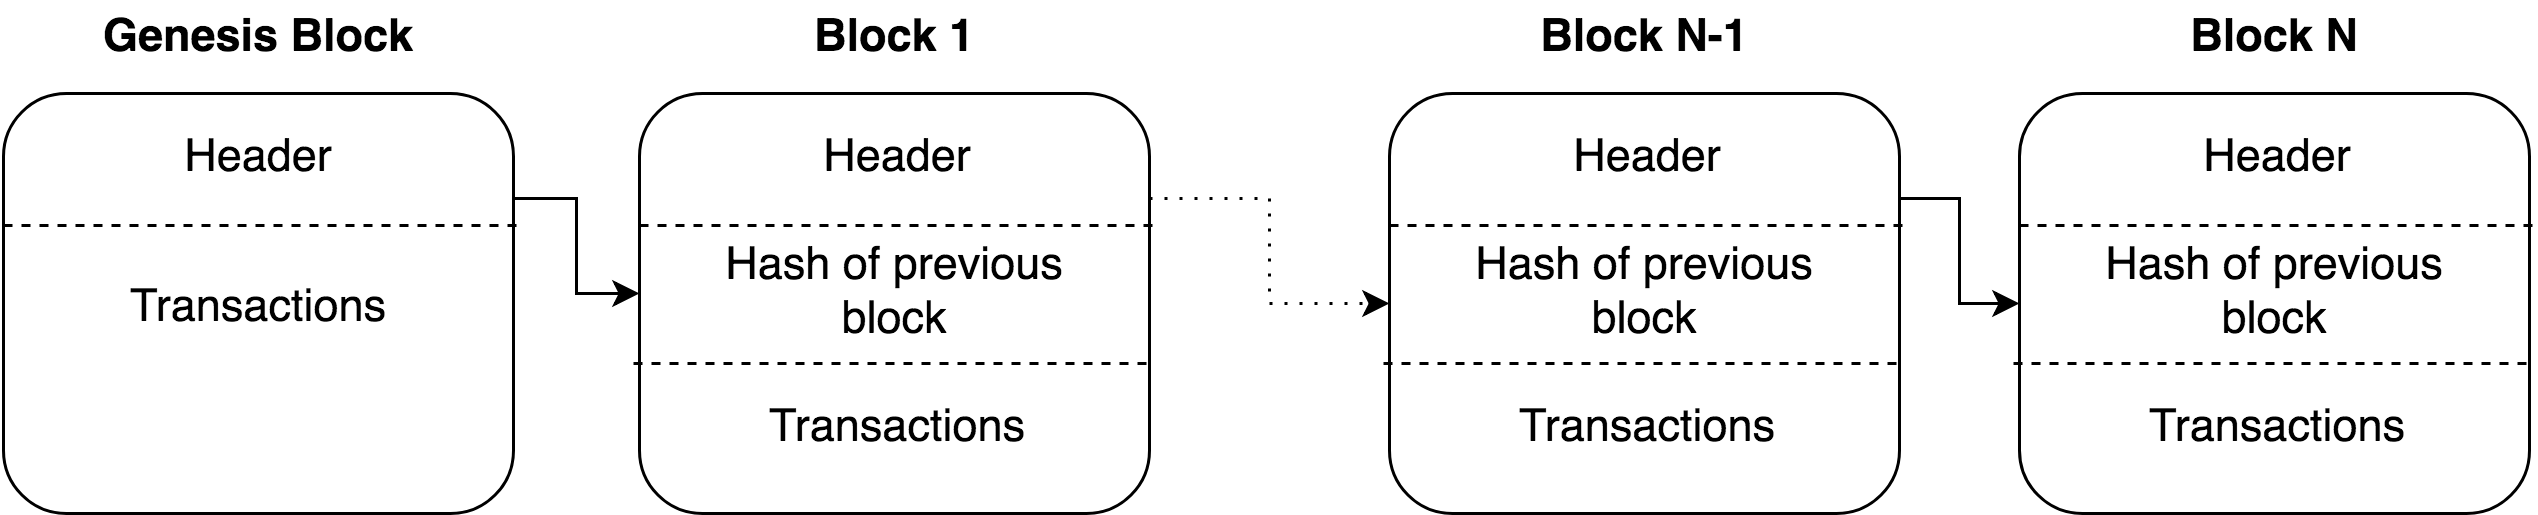
\includegraphics[width=1\textwidth]{images/blockchain_simplified.png}
% 	    \caption{Blockchain simplified }
% 	    \label{fig:block_simpl}
% 	\end{figure}
% \subsection{Accessibility}
% A blockchain can be defined as an immutable shared ledger that holds transactions, maintained within a decentralized and distributed network of mutually non-trusting peers. Every peer maintains their copy of the ledger and is responsible of validating each transaction on it.

% \subsubsection{Permissionless vs Permissioned}
% At permissionless or else public blockchains anyone can participate. Parties are mutually untrusted and for the network to be stable and robust we need economic incentives through mining. 

% Permissioned chains or private chains accept only whitelisted member or else known members. Because members are known in that network we have a legal incentive and reputation as well, thus all players are honest. For this reason we don't need mining to keep an honest network, thus we can easily achieve higher transaction throughput and less energy consumption, we also don't need a cryptocurrency for this network to work.

% \subsection{UTXO and Balance Model}
% %https://ethereum.stackexchange.com/questions/326/what-are-the-pros-and-cons-of-ethereum-balances-vs-utxos
% %benefits